\begin{figure*}
  \centering
  \begin{subfigure}[b]{0.05\textwidth}
    ~
  \end{subfigure}
  % 
  \begin{subfigure}[b]{0.45\textwidth}
    \centering
    ~~\textbf{Mild plate effects}
  \end{subfigure}
  % 
  \begin{subfigure}[b]{0.45\textwidth}
    \centering
    ~~\textbf{Strong plate effects}
  \end{subfigure}

  \begin{subfigure}[c]{0.05\textwidth}
    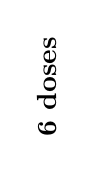
\begin{tikzpicture}
      \node[rotate=90] {\textbf{6 doses}};  
    \end{tikzpicture}
  \end{subfigure}  
  % 
  \begin{subfigure}[c]{0.45\textwidth}
    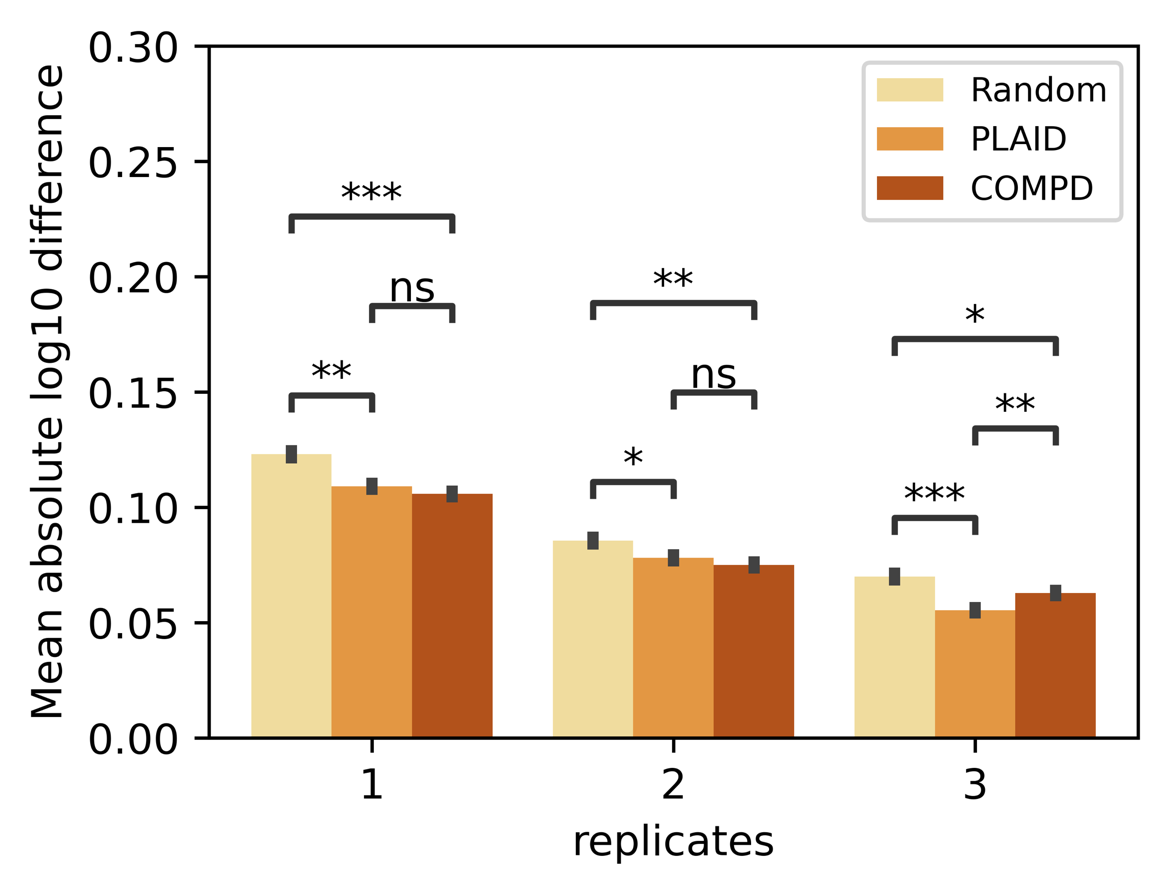
\includegraphics[width=\textwidth]{figures/dose-response-absic50-1-2-3-6doses-dil18-bowl-0.055.png}
  \end{subfigure}
  %
  \begin{subfigure}[c]{0.45\textwidth}
    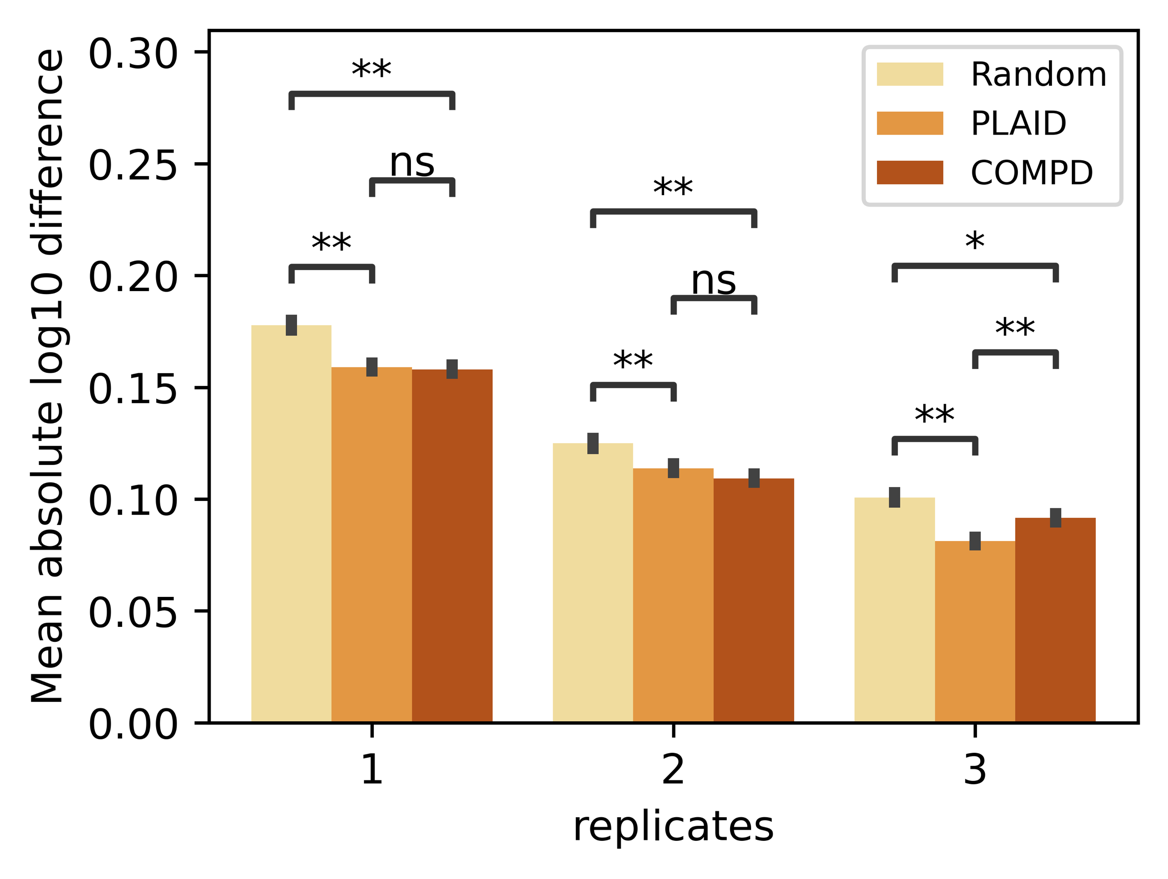
\includegraphics[width=\textwidth]{figures/dose-response-absic50-1-2-3-6doses-dil18-bowl-0.085.png}
  \end{subfigure}

  \begin{subfigure}[c]{0.05\textwidth}
    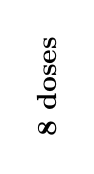
\begin{tikzpicture}
      \node[rotate=90] {\textbf{8 doses}};  
    \end{tikzpicture}
  \end{subfigure}  
  %
  \begin{subfigure}[c]{0.45\textwidth}
    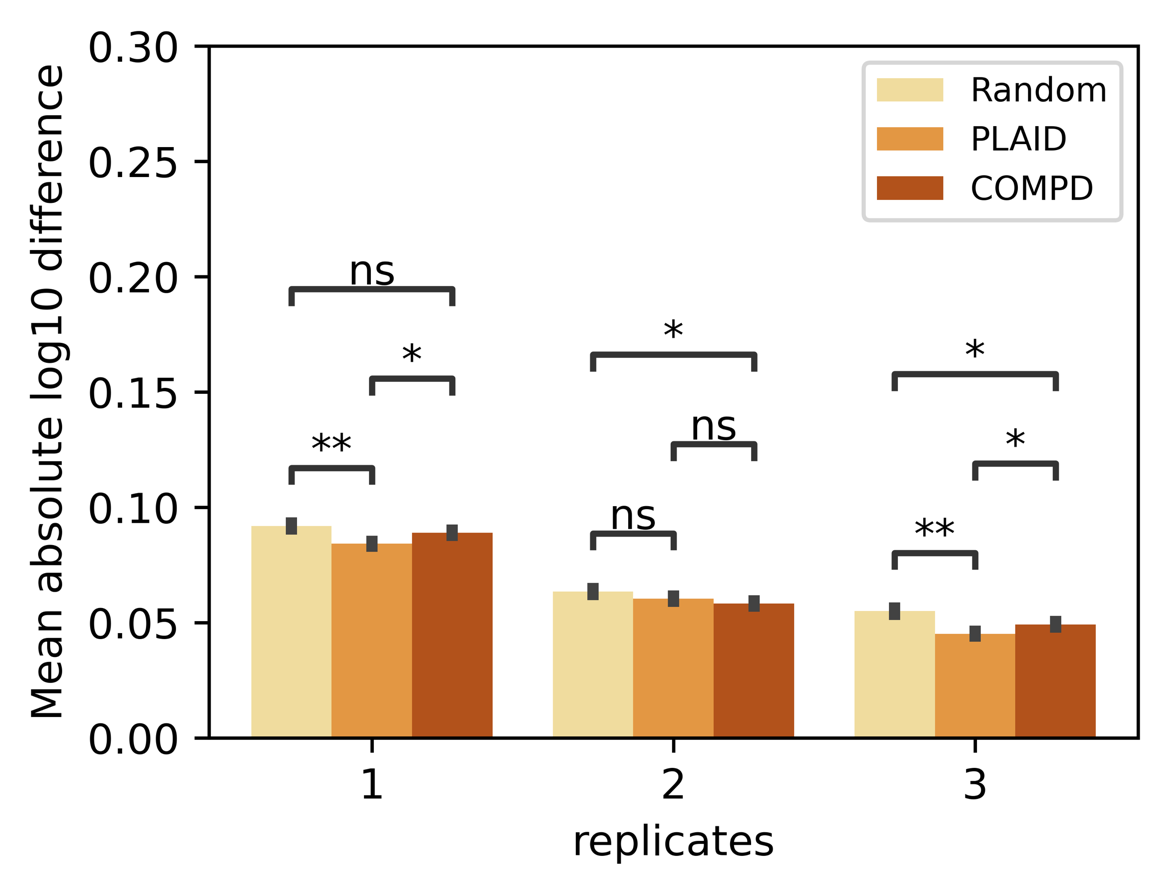
\includegraphics[width=\textwidth]{figures/dose-response-absic50-1-2-3-8doses-dil8-bowl-0.055.png} 
  \end{subfigure} 
  %
  \begin{subfigure}[c]{0.45\textwidth}
    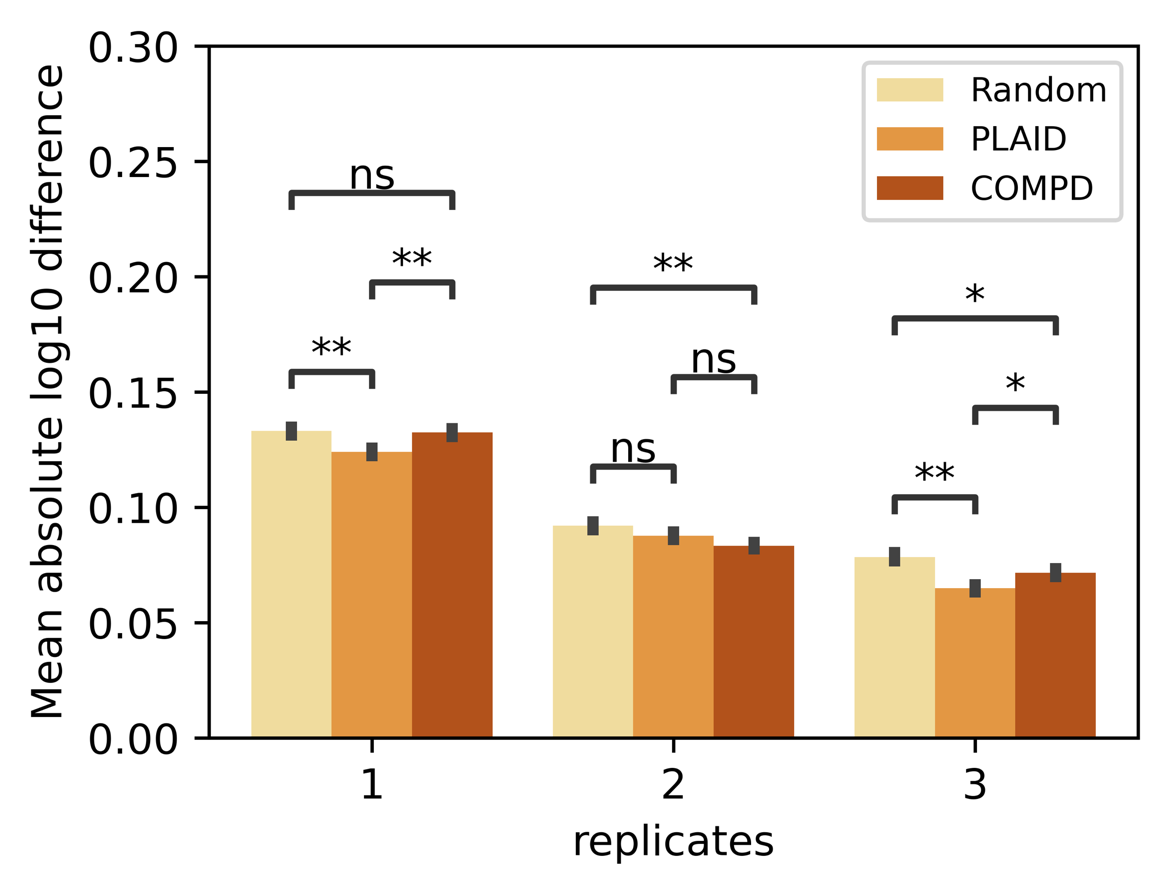
\includegraphics[width=\textwidth]{figures/dose-response-absic50-1-2-3-8doses-dil8-bowl-0.085.png}
  \end{subfigure}

  \begin{subfigure}[c]{0.05\textwidth}
    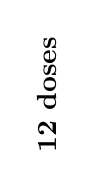
\begin{tikzpicture}
      \node[rotate=90] {\textbf{12 doses}};  
    \end{tikzpicture}
  \end{subfigure}  
  %
  \begin{subfigure}[c]{0.45\textwidth}
    \includegraphics[width=\textwidth]{figures/dose-response-absic50-1-2-3-12doses-dil4-bowl-0.055.png}
  \end{subfigure} 
  %
  \begin{subfigure}[c]{0.45\textwidth}
    \centering
     \includegraphics[width=\textwidth]{figures/dose-response-absic50-1-2-3-12doses-dil4-bowl-0.085.png}
  \end{subfigure}
  \caption{Mean absolute $\log_{10}$ difference between expected and
    obtained values of the absolute
    {$\text{EC}_{50}$/$\text{IC}_{50}$} for dose-response curves using
    various numbers of doses, replicates, and bowl-shaped plate-effect
    strengths. The 4PL sigmoide curves were fitted using only compound
    data. *** indicates $p<10^{-43}$.}
\end{figure*}


%%% Local Variables: 
%%% mode: latex
%%% TeX-master: "../supplement.tex"
%%% End: 